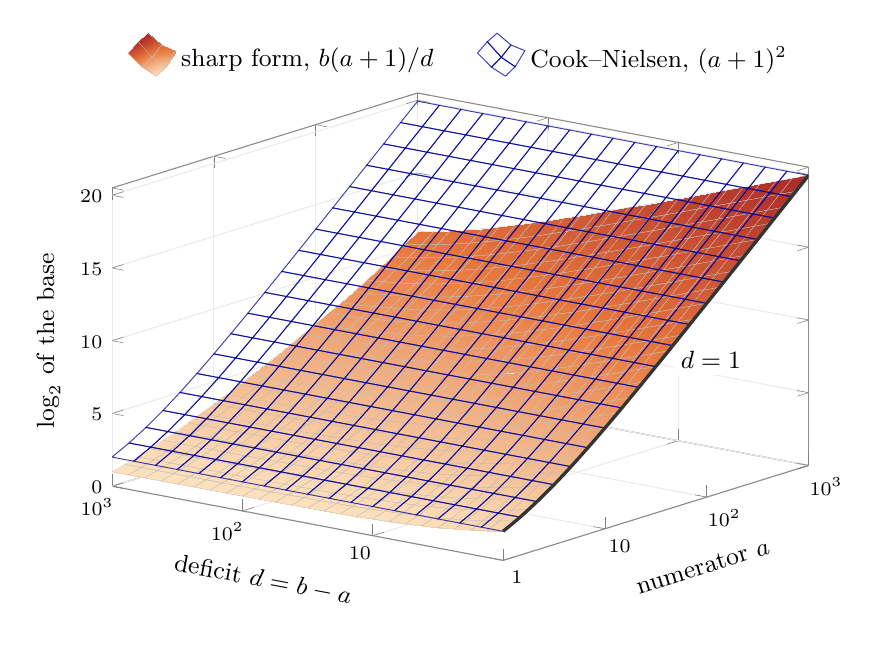
\begin{tikzpicture}
\begin{axis}[width=0.86\textwidth, height=0.62\textwidth, view={-52}{22},
  xmin=0, xmax=3, ymin=0, ymax=3, zmin=0, zmax=20.5,
  xtick={0,1,2,3}, xticklabels={$1$,$10$,$10^2$,$10^3$},
  ytick={0,1,2,3}, yticklabels={,$10$,$10^2$,$10^3$},
  ztick={0,5,10,15,20},
  tick label style={font=\scriptsize}, label style={font=\small},
  xlabel={numerator $a$}, ylabel={deficit $d=b-a$},
  zlabel={$\log_2$ of the base},
  xlabel style={sloped like x axis, yshift=2pt}, ylabel style={sloped like y axis, yshift=2pt},
  grid=major, grid style={black!8}, axis line style={black!45},
  colormap={warm}{rgb255=(253,226,190) rgb255=(232,120,60) rgb255=(170,40,40)},
  legend image post style={line width=0.8pt}, legend style={at={(0.5,1.02)}, anchor=south, legend columns=2, draw=none, font=\small,
    /tikz/every even column/.append style={column sep=14pt}}]
% base b(a+1)/d of the sharp product lemma
\addplot3[surf, domain=0:3, y domain=0:3, samples=25, samples y=25,
  shader=faceted interp, faceted color=black!25, line width=0.1pt, point meta=z]
  {ln((10^x+10^y)*(10^x+1)/10^y)/ln(2)};
\addlegendentry{sharp form, $b(a+1)/d$}
% Cook--Nielsen base (a+1)^2: drawn as a wire mesh above the solid sheet
\addplot3[mesh, domain=0:3, y domain=0:3, samples=19, samples y=19,
  draw=blue!60!black, line width=0.35pt, draw opacity=0.75]
  {2*ln(10^x+1)/ln(2)};
\addlegendentry{Cook--Nielsen, $(a+1)^2$}
% the two sheets meet along d = 1
\addplot3[very thick, black!80, domain=0:3, samples=40, samples y=1] (x, 0, {2*ln(10^x+1)/ln(2)});
\node[font=\small, anchor=west, fill=white, inner sep=2pt, xshift=5pt] at (axis cs:1.55,0,{2*ln(10^1.55+1)/ln(2)}) {$d=1$};
\end{axis}
\end{tikzpicture}
